\chapter{Matrizen und lineare Abbildungen}

\section{Definition: Darstellungsmatrix}
	Seien $V,W$ endlich dimensionale $K$-Vektorräume und $\mathcal{B}=\lrr{v_1,\dots,v_n}$ und\\
	$\varphi=\lrr{w_1,\dots,w_m}$ geordnete Basen von $V$ beziehungsweise $W$.\\
	Sei $\alpha: V\rightarrow W$ eine lineare Abbildung.\\
	Nach 4.10 ist $\alpha$ eindeutig bestimmt durch $\alpha\lrr{v_1},\dots,\alpha\lrr{v_n}$.\\
	Stelle $\alpha\lrr{v_1}$ bezüglich der BAsis $\varphi$ dar, $i=1,\dots,n$\\
	$\begin{array}{l}
		\alpha\lrr{v_1}=a_{11}w_1+\dots+a_{m1}w_m\\
		\vdots\\
		\alpha\lrr{v_n}=a_{1n}w_1+\dots+a_{mn}w_m
	\end{array}$\\
	Dann heißt die $m\times n$-Matrix \textbf{Darstellungsmatrix} von $\alpha$ bezüglich $\mathcal{B}$ und $\varphi$

	$A_{\alpha}^{\mathcal{B}, \varphi}:=\lrv{a_{11}&a_{12}&\dots&a_{1n}\\\vdots&\vdots&\ddots&\vdots\\a_{m1}&a_{m2}&\dots&a_{mn}}$

	In den Spalten stehen die Koordinaten von $\alpha\lrr{v_i}$ bezüglich $\varphi, i=1,\dots,n$\\
	Beachte: Wenn $A_{\alpha}^{\mathcal{B}, \varphi}$ und $\mathcal{B},\varphi$ bekannt sind, dann ist $\alpha$ vollständig bestimmt.\\
	Abkürzende Schreibweise:\\
	$A_\alpha$ statt $A_{\alpha}^{\mathcal{B}, \varphi}$, wenn $\mathcal{B},\varphi$ aus Kontext ersichtlich sind.\\
	Falls $V=W$ und $\mathcal{B}=\varphi$: $A_{\alpha}^{\mathcal{B}}$ statt $A_{\alpha}^{\mathcal{B}, \mathcal{B}}$

\section{Beispiel}
	$V=W=\mr^2$, $\mathcal{B}$ ist kanonische Basis. $A_\alpha^{\mathcal{B}}=\lrv{1&2\\3&4}$\\
	Was ist $\alpha\lrr{\lrv{2\\3}}$?\\
	$\alpha\lrr{\lrv{1\\0}}=1\lrv{1\\0}+3\lrv{0\\1}=\lrv{1\\3}$\\
	$\alpha\lrr{\lrv{0\\1}}=\lrv{2\\4}$\\
	$\alpha\lrr{\lrv{2\\3}}=\alpha\lrr{2\cdot\lrv{1\\0}+3\cdot\lrv{0\\1}}=2\cdot\alpha\lrr{\lrv{1\\0}}+3\alpha\lrr{\lrv{0\\1}}=2\cdot\lrv{1\\3}+3\cdot\lrv{2\\4}=\lrv{8\\18}$

\section{Bemerkung}
	\subExBegin{a)}
		\item Nach 5.1 ist $\alpha$ durch $A_{\alpha}^{\mathcal{B}, \varphi}$ eindeutig bestimmt:\\
			$\mathcal{B},\varphi$ wie in 5.1, $\alpha:V\rightarrow W$.\\
			$v\in V, v=\limsum{i=1}{n}c_iv_i$, also ist\\
			$\alpha\lrr{v}=\limsum{i=1}{n}c_i\alpha\lrr{v_i}=\limsum{i=1}{n}c_i\lrr{\limsum{j=1}{m}a_{ji}w_j}=\limsum{j=1}{m}\underbrace{\lrr{\limsum{i=1}{n}a_{ji}c_i}}_{\mbox{\scriptsize Koord. }\scriptstyle \alpha(v)\mbox{\scriptsize \;bzgl. }\scriptstyle\varphi}w_j$
		\item Ist $A=\lrv{a_{11}&\dots&a_{1n}\\\vdots&&\vdots\\a_{m1}&\dots&a_{mn}}$ eine $m\times n$-Matrix über $K$.\\
			Dann existiert genau eine lineare Abbildung $\alpha:V\rightarrow W$ mit $A_{\alpha}^{\mathcal{B}, \varphi}=A$\\
			Das heißt jede $m\times n$-Matrix tritt als Darstellungsmatrix einer linearen Abbildung bezüglich vorgegebenen Basen $\mathcal{B}$ und $\varphi$ auf.

			Setze $w_i'=a_{1i}w_1+a_{2i}w_2+\dots+a_{mi}w{m}$, mit $i=1,\dots,n$, dann existiert nach 4.10 genau eine lineare Abbildung $\alpha:V\rightarrow W$ mit $\alpha\lrr{v_i}=w_i'$ für $i=1,\dots,n$\\
			Dann $A_{\alpha}^{\mathcal{B}, \varphi}=A$
		\item Dieselbe lineare Abbildung hat im Allgemeinen bezüglich anderer Wahl der Basen eine andere Darstellungsmatrix.
	\subExEnd

\section{Beispiele}
	\subExBegin{a)}
		\item $V=\mr^2=W, \mathcal{B}=\varphi$ kanonische Basis von $\mr^2$, $\alpha$ Drehung im Nullpunkt um den Winkel $\varphi$ gegen den Uhrzeigersinn.\\
			4.11:$\alpha\lrr{e_1}=\cos\lrr{\varphi}e_1+\sin\lrr{\varphi}e_2$\\
			$\alpha\lrr{e_2}=-\sin\lrr{\varphi}e_1+\cos\lrr{\varphi}e_2$

			$A_{\alpha}^{\mathcal{B}}=\underset{\mbox{\scriptsize Drehmatrix}}{\lrv{\cos\lrr{\varphi}&-\sin\lrr{\varphi}\\\sin\lrr{\varphi}&\cos\lrr{\varphi}}}$
		\item $\alpha:V\rightarrow W$ Nullabbildung hat bezüglich jeder Wahl von $\mathcal{B},\varphi$ die Nullmatrix als Darstellungsmatrix.
		\item $\id_V:V\rightarrow V$, $\mathcal{B}$ Basis von $V$\\
			$A_{\id_V}^{\mathcal{B}}=\lrv{1&0&\dots&0\\&&\\0&\dots&1}=E_n$ mit $\dim\lrr{V})n$
		\item zweidimensionales $V$ mit $v_1,v_2,\varphi=\lrv{v_2\\v_1}$\\
			$A_{\id_V}^{\mathcal{B},\varphi}=\lrv{0&1\\1&0}$
		\item $V=\mr^2,\mathcal{B}=\lrr{e_1,e_2}$ kanonische Basis, $\sigma$ Spiegelung an $\left\langle e_1\right\rangle$

      \begin{tikzpicture}[scale=1.5]
        \draw [-] (-2,0) -- (2,0);
        \draw [-] (0,-2) -- (0,2);
        \draw [thick,->] (0,0) -- (1,0) node [anchor=south west] {$e_1$};
        \draw [dotted] (1,-1) node [anchor=west] {$\sigma(v)$} -- (1,1) node [anchor=west] {$v$};
        \draw [thick,->] (0,0) -- (0,1) node [anchor=east] {$e_2$};
        \draw [thick,->] (0,0) -- (0,-1) node [anchor=east] {$-e_2$};
        \draw [->] (0,0) -- (1,1) node [anchor=south] {$\scriptstyle e_1+e_2$};
        \draw [->] (0,0) -- (1,-1) node [anchor=north] {$\scriptstyle e_1-e_2$};
      \end{tikzpicture}

			$A_{\sigma}^{\mathcal{B}}=\lrv{1&0\\0&-1}$\\
			$\sigma\lrr{\lrv{x_1\\x_2}}=\lrv{x_1\\-x_2}=\lrv{1&0\\0&-1}\lrv{x_1\\x_2}$\\
			$\mathcal{B}'=\lrr{e-1+e_2, e_1-e_2}=\lrr{\lrv{1\\1},\lrv{1\\-1}}$\\
			$A_\sigma^{\mathcal{B}'}=\lrv{0&1\\1&0}$\\
			$\sigma\lrr{e_1+e_2}=e_1-e_2=0\cdot\lrr{e_1+e_2}+1\cdot\lrr{e_1-e_2}$\\
			$\sigma\lrr{e_1-e_2}=e_1+e_2=1\cdot\lrr{e_1+e_2}+0\cdot\lrr{e_1-e_2}$

			$A_\sigma^{\mathcal{B},\mathcal{B}'}$\\
			$\sigma\lrr{e_1}=\underline{e_1}=a_{11}\lrr{e_1+e_2}+a_{21}\lrr{e_1-e_2}=\underline{\lrr{a_{11}+a_{21}}e_1+\lrr{a_{11}-a_{21}}e_2}$\\
			$\sigma\lrr{e_2}=\underline{-e_2}=a_{12}\lrr{e_1+e_2}+a_{22}\lrr{e_1-e_2}=\underline{\lrr{a_{12}+a_{22}}e_1+\lrr{a_{12}-a_{22}}e_2}$\\
			$a_{11}+a_{21}=1\quad a_{11}-a_{21}=0\Rightarrow a_{11}=a_{21}=\frac{1}{2}$\\
			$a_{12}+a_{22}=0\quad a_{12}-a_{22}=-1\Rightarrow a_{12}=-\frac{1}{2},a_{22}=\frac{1}{2}$\\
			$A_\sigma^{\mathcal{B},\mathcal{B}'}=\lrv{\frac{1}{2}&-\frac{1}{2}\\\frac{1}{2}&\frac{1}{2}}$
	\subExEnd

\section{Satz: Koordinatenvektor}
	$V,W$ sind endlich dimensionale $K$-Vektorräume, $\mathcal{B},\varphi$ geordnete Basen von $V$\\
	beziehungsweise $W$, $\alpha:V\rightarrow W$ eine lineare Abbildung.\\
	Sei $v\in V$, $k_{\mathcal{B}}\lrr{v}$ der Koordinatenvektor von $v$ bezüglich $\mathcal{B}$.\\
	Der Koordinatenvektor von $\alpha\lrr{v}$ bezüglich $\varphi$ lässt sich berechnen als\\
	$k_\varphi\lrr{\alpha\lrr{v}}=A_{\alpha}^{\mathcal{B},\varphi}\cdot k_\mathcal{B}\lrr{v}$

  \begin{tikzpicture}
    \draw [<-,thick] (0,0) node [anchor=north east] {$\scriptstyle K^n$} -- node [anchor=east] {$K_\mathcal{B}$} (0,2) node [anchor=south east] {$\scriptstyle\overset{\mathcal{B}}{V}$};
    \draw [->,thick] (0,2) -- node [anchor=south] {$\alpha$} (2,2) node [anchor=south west] {$\scriptstyle\overset{\varphi}{W}$};
    \draw [->,thick] (2,2) -- node [anchor=west] {$\scriptstyle K_l$} (2,0) node [anchor=north west] {$\scriptstyle K^m$};
    \draw [->,thick] (0,0) -- node [anchor=south] {$A_\alpha^{\mathcal{B},l}$} (2,0);
  \end{tikzpicture}

	\textbf{Beweis} - Folgt aus 5.3a)

\section{Beispiel}
	$V,W$ seien $\mr$-Vektorräume mit $\dim\lrr{V}=4, \dim\lrr{W}=3$ und $\mathcal{B}=\lrr{v_1,\dots,v_4},\varphi=\lrr{w_1,w_2,w_3}$, $\alpha:V\rightarrow W$ linear mit \\
	$A_\alpha^{\mathcal{B},\varphi}=\lrv{1&1&2&3\\2&0&-1&1\\3&2&0&2}$\\
	$v=5v-1-6v_2+7v_3-2v_4$, $\alpha\lrr{v}=?$\\
	5.5:$\lrv{1&1&2&3\\2&0&-1&1\\3&2&0&2}\lrv{5\\-6\\7\\-2}=\lrv{7\\1\\-1}$\\
	$\alpha\lrr{v}=7w_1+w_2-w_3$

\section{Korollar: Darstellung linearer Abbildungen}
	Jede lineare Abbildung $K^n\rightarrow K^m$ ist von der Form $\alpha\lrr{x}=A\cdot x$ für eine $m\times n$-Matrix $A$ über $K$.

	\textbf{Beweis:}\\
	Die Elemente von $K^n$ ($K^m$) stimmen mit ihren Koordinatenvektoren bezüglich der kanonischen Basen überein. Behauptung folgt mit 5.5

\section{Satz: Rechenregeln}
	$\alpha,\beta$ lineare Abbildungen $U\rightarrow V$\\
	$\gamma$ lineare Abbildung $V\rightarrow W$

	$\mathcal{B},\varphi,\mathcal{D}$ geordnete Basen von $U,V,W$
	\begin{enumerate}[a)]
		\item $A_{\alpha+\beta}^{\mathcal{B},\varphi}=A_\alpha^{\mathcal{B},\varphi}+A_\beta^{\mathcal{B},\varphi}$\\
			$A_{k\alpha}^{\mathcal{B},\varphi}=k\cdot A_\alpha^{\mathcal{B},\varphi}$ ($k\in K$)

		\item $A_{\gamma\circ\alpha}^{\mathcal{B},\mathcal{D}}=A_\gamma^{\varphi,\mathcal{D}}\cdot A_\alpha^{\mathcal{B},\varphi}$ gleiche Basis
	\end{enumerate}
	\textbf{Beweis:}
	\begin{enumerate}[a)]
		\item Nachrechnen
		\item $A_\alpha^{\mathcal{B},\varphi}=(a_{ij})$, $A_\gamma^{\varphi,\mathcal{B}}=(b_{ij})$\\
			$\mathcal{B}=(u_1,...,u_l)$\\
			$\varphi=(v_1,...,v_m)$\\
			$\mathcal{D}=(w_1,...,w_n)$\\
			$(\gamma\circ\alpha)(u_i)=\gamma(\alpha(u_i))=\gamma\lrr{\limsum{j=1}{m}a_{ij}v_j}=\limsum{j=1}{m}a_{ij}\cdot\gamma(v_j)=\limsum{j=}{m}a_{ij}\lrr{\limsum{k=1}{n}b_{jk}w_k}=\limsum{k=1}{n}\underbrace{\lrr{\limsum{j=1}{m}b_{kj}a_{ji}}}_{\mbox{Koeff.} (k,i)\mbox{ in }A_\gamma^{\varphi,\mathcal{D}}\cdot A_\alpha^{\mathcal{B},\varphi}}w_k$
	\end{enumerate}

\section{Beispiel}
	$V=\mr^2, B=\lrr{e_1,e_2}$ kanonische Basis, $\alpha: V\rightarrow V, \beta V\rightarrow V$\\
	Dabei stellt $\alpha$ bzw. $\beta$ eine Drehung um den Winkel $\varphi$ bzw. $\psi$ um den Nullpunkt dar.

	5.4a) $A_\alpha^B=\lrv{\cos\lrr{\varphi}&-\sin\lrr{\varphi}\\\sin\lrr{\varphi}&\cos\lrr{\varphi}}$\\
	$A_\beta^B=\lrv{\cos\lrr{\psi}&-\sin\lrr{\psi}\\\sin\lrr{\psi}&\cos\lrr{\psi}}$\\
	$\beta\circ\alpha =$ Drehung um $\phi+\psi$\\
	$A_{\scriptstyle\beta\circ\alpha}^B=\lrv{\cos\lrr{\varphi+\psi}&-\sin\lrr{\varphi+\psi}\\\sin\lrr{\varphi+\psi}&\cos\lrr{\varphi+\psi}}$\\
	Nach 5.8b) gilt $A_{\scriptstyle\beta\circ\gamma}^B=A_\beta^B\cdot A_\alpha^B=\lrv{\cos\lrr{\varphi}\cos\lrr{\psi}-\sin\lrr{\varphi}\sin\lrr{\psi}&-\cos\lrr{\psi}\sin\lrr{\varphi}-\sin\lrr{\psi}\cos\lrr{\varphi}\\
	\cos\lrr{\varphi}\sin\lrr{\psi}+\sin\lrr{\varphi}\cos\lrr{\psi}&-\sin\lrr{\varphi}\sin\lrr{\psi}+\cos\lrr{\varphi}\cos\lrr{\psi}}$\\
	$\Rightarrow$\\
	$\cos\lrr{\varphi+\psi}=\cos\lrr{\varphi}\cos\lrr{\psi}-\sin\lrr{\varphi}\sin\lrr{\psi}$\\
	$\sin\lrr{|varphi+\psi}=\cos\lrr{\varphi}\sin\lrr{\psi}+\sin\lrr{\varphi}\cos\lrr{\psi}$\\
	\textbf{Additionstheoreme} für $\sin,\cos$

\section{Korollar: Matrizen invertieren}
	$\dim_k\lrr{V}=n$, $B$ Basis von $V$, $\alpha:V\rightarrow V$ linear.\\
	$\alpha$ ist invertierbar $\Leftrightarrow A_\alpha^B$ ist invertierbar\\
	Dann gilt $A_{\alpha^{-1}}^B=\lrr{A_\alpha^B}^{-1}$

	\textbf{Beweis}
	\begin{enumerate}
		\item[$\Rightarrow$:] $\alpha^{-1}:V\rightarrow V$ existiert, $\alpha\circ\alpha^{-1}=\alpha^{-1}\circ\alpha=\id_V$\\
			$A_\alpha^B\cdot A_{\alpha^{-1}}^B\underset{\mbox{\scriptsize  5.8b)}}{=} A_{\id_V}^B =E_n = A_{a^{-1}}^B\cdot A_\alpha^B$\\
			$\lrr{A_\alpha^B}^{-1}=A_{\alpha^{-1}}^B$
		\item[$\Leftarrow$:] $A_\alpha^B\cdot B=B\cdot A_\alpha^B=E_n$\\
			Dann ist $B=A_\beta^B$ für eine eindeutig bestimmte lineare Abbildung $\beta:V\rightarrow V$ (5.3b))\\
			Nach 5.8 gilt $A_\alpha^B\cdot A_\beta^B=A_\beta^B\cdot A_\alpha^B=E_n$\\
			$A_{\alpha\circ\beta}^B=A_{\beta\circ\alpha}^B=A_{\id_V}^B$\\
			Folglich gilt $\alpha\circ\beta=\beta\circ\alpha=\id_V$, $\alpha$ invertierbar $\beta =\alpha^{-1}$
	\end{enumerate}

\section{Satz: Invertierbarkeit}
	Sei $A$ eine $n\times n$-MAtrix über $K$.\\
	Dann gilt $A$ ist invertierbar $\Leftrightarrow\rg(A)=n$\\
	Das heist alle Zeilen von $A$ sind linear unabhängig bzw. alle Spalten von $A$ sind linear unabhängig.

	\textbf{Beweis}

	Sei $\alpha:K^n\rightarrow K^n$ definiert durch $\alpha(x)=A\cdot x$, $x\in K^n$\\
	$A=A_\alpha^B$, $B$ ist kanonische Basis.\\
	$A$ invertierbar $\ouset{\Leftrightarrow}{}{\mbox{\scriptsize 5.10}}\alpha$ invertierbar $\ouset{\Leftrightarrow}{}{\mbox{\scriptsize 4.16}}\alpha$ surjektiv $\rg\lrr{\alpha}=n\ouset{\Leftrightarrow}{}{\mbox{\scriptsize 4.18}}\rg\lrr{A}=n$

\section{Lemma}
	$A\in M_{m,n}\lrr{K}, X\in M_{n,l}\lrr{K}, C=AX\in M_{m,l}\lrr{K}$\\
	Wendet man auf $A$ und $C$ die gleichen elementaren Zeilenumfromungen an, so gilt für die entstehenden Matrizen $A'$ und $C'$ $A'X=C'$

	\textbf{Beweis}

	$AX=C\Leftrightarrow AX_i=C_i$ wobei $i$ der Spaltenindex ist.

\section{Bestimmung von \texorpdfstring{$A^{-1}$ für invertierbare $n\times n$- Matrix $A$}{invertierbarer Matrix}}
	Sei $A$ eine invertierbare $n\times n$ Matrix.\\
	Suche $A^{-1}$ $n\times n$-Matrix mit $A\cdot A^{-1}=E_n$.\\
	$A$ kann man durch elementare Zeilenumfromungen in $E_n$ umwandeln. \\
	Wie bei Gauß. Zusätzlich auch oberhalb der Diagonalen in jeder Spalte Nullen erzeugen und Diagonalelemente zu $1$ machen (Multiplikation mit $a^{-1}$ falls $a$ in Diagonale steht)\\
	Funktioniert, da $\rg(A)=n$

	$A\cdot A^{-1} =E_n$\\
	Elementare Zeilenumformungen an $A\rightarrow E_n$, selbe elementare Umformunan an $E_n$ durchführen.\\
	$A\cdot A^{-1} =E_n$\\
	$E_n\cdot A^{-1} = B$ das heist $B=A^{-1}$

	$\lrv{A&E_n}\rightarrow\lrv{E_n&A^{-1}}$

\section{Beispiel}
	$A=\lrv{1&0&2\\2&2&1\\0&1&0}, K=\mq$

	$\lrv{1&0&2&1&0&0\\2&2&1&0&1&0\\0&1&0&0&0&1}\rightarrow\lrv{1&0&2&1&0&0\\0&2&-3&-2&1&0\\0&1&0&0&0&1}\rightarrow\lrv{1&0&2&1&0&0\\0&1&-\frac{1}{2}&-1&\frac{1}{2}&0\\0&1&0&0&0&1}\rightarrow\lrv{1&0&2&1&0&0\\0&1&-\frac{3}{2}&-1&\frac{1}{2}&0\\0&0&\frac{3}{2}&1&-\frac{1}{2}&1}\rightarrow
	\lrv{1&0&2&1&0&0\\0&1&0&0&0&1\\0&0&1&\frac{2}{3}&-\frac{1}{3}&\frac{2}{3}}\rightarrow\lrv{1&0&0&-\frac{1}{3}&\frac{2}{3}&-\frac{4}{3}\\0&1&0&0&0&1\\0&0&1&\frac{2}{3}&-\frac{1}{3}&\frac{2}{3}}$

	Der rechte Teil entspricht $A^{-1}$

\section{Definition: Basiswechselmatrix}
	Sei $V$ ein $K$-Vektorraum und $B=\lrv{v_1,\dots,v_n}, B'=\lrv{v_1',\dots,v_n'}$ Basen

	$v_j'=\limsum{i=1}{n}s_{ij}v_i, j=1,\dots,n$\\
	$S_{B,B'}=\lrr{s_{ij}}_{\scriptstyle i,j=1,\dots,n}$ heist \textbf{Basiswechselmatrix}

	Die Spalten entsprechen den Koordinaten der Basisvektoren in $B'$ bezüglich $B$\\
	Analog: $v_k=\limsum{j=1}{n}t_{jk}v_j', k=1,\dots, n$\\
	$S_{B',B}=\lrr{t_{jk}}_{\scriptstyle j,k=1,\dots,n}$

\section{Satz}
	Bezeichnungen gelten wie in 5.15.\\
	$S_{B,B'}$ ist invertierbar, $\lrr{S_{B,B'}}^{-1}=S_{B',B}$\\
	$S_{B,B'}\cdot S_{B',B}=S_{B',B}\cdot S_{B,B'}=E_n$

	\textbf{Beweis}

	$v_k=\limsum{j=1}{n}t_{jk}v_j'=\limsum{j=1}{n}t_{jk}\lrr{\limsum{i=1}{n}s_{ij}v_i}=\limsum{i=1}{n}\lrr{\limsum{j=1}{n}s_{ij}t_{jk}}v_i, k=1,\dots,n$\\
	$\Rightarrow\limsum{j=1}{n}s_{ij}t_{jk}=\begin{cases}0,i\neq k\\1,i=k\end{cases}, k=1,\dots,n$\\
	$S_{B,B'}\cdot S_{B',B}=E_n$

	Andere Richtung funktioniert analog.

\section{Korollar}
	Seien $V,B,B'$ wie oben definiert, $v\in V$\\
	Dann gilt $k_{B'}\lrr{v}=S_{B',B}\cdot k_B{v}$

	\textbf{Beweis}

	$v=\sum c_iv_i, k_B(v)=\lrv{c_1\\\vdots\\c_n}$\\
	$V=\limsum{i=1}{n}c_i\lrr{\limsum{j=1}{n}t_{ji}v_j'}=\limsum{j=1}{n}\lrr{\limsum{i=1}{n}t_{ij}c_i}v_j'$\\
	Behauptung folgt.

\section{Beispiel}
	$V=\mr^2, B=\lrr{e_1,e_2}$ kanonische Basis, $B'=\lrr{e_1+e_2,e_1-2e_2}$ Basis\\
	$S_{B,B'}=\lrv{1&1\\1&-2}$\\
	$S_{B',B}=S_{B,B'}^{-1}$ nach 5.16.\\
	Bestimme $\lrv{1&1\\1&-2}^{-1}$ nach 5.14:\\
	$\lrv{1&1&1&0\\1&-2&0&1}\rightarrow\lrv{1&1&1&0\\0&-3&-1&1}\rightarrow\lrv{1&1&1&0\\0&1&\frac{1}{3}&-\frac{1}{3}}\rightarrow\lrv{1&0&\frac{2}{3}&\frac{1}{3}\\0&1&\frac{1}{3}&-\frac{1}{3}}$\\
	$S_{B',B}=\lrv{\frac{2}{3}&\frac{1}{3}\\\frac{1}{3}&-\frac{1}{3}}$\\
	$e_1=\frac{2}{3}\lrr{e_1+e_2}+\frac{1}{3}\lrr{e_1-2e_2}$\\
	$e_2=\frac{1}{3}\lrr{e_1+e_2}-\frac{1}{3}\lrr{e_1-2e-2}$

	Sei $v=\lrv{5\\3}=k_B\lrr{v}$\\
	$k_{B'}(v)\ouset{=}{}{\smt{5.17}}\lrv{\frac{2}{3}&\frac{1}{3}\\\frac{1}{3}&-\frac{1}{3}}\cdot\lrv{5\\3}=\lrv{\frac{13}{3}\\\frac{2}{3}}$\\
	Das heist $v=\frac{13}{3}\lrr{e_1+e_2}+\frac{2}{3}\lrr{e_1-2e_2}$\\
	$\lrv{5\\3}=\frac{13}{3}\lrv{1\\1}+\frac{2}{3}\lrv{1\\-2}$

\section{Satz}
	$\alpha:V\rightarrow W$ linear, $V,W$ sind $K$-Vektorräume\\
	$B,B'$ sind geordnete Basen von $V$, $\varphi,\varphi'$ sind geordnete Basen von $W$.

	Dann: $A_\alpha^{B',\varphi'}=S_{\varphi',\varphi}\cdot A_\alpha^{B,\varphi}\cdot S_{B,B'}$

	\textbf{Beweis}

	Sei $v\in V$\\
  $A_\alpha^{B',\varphi'}\cdot k_{B'}\lrr{v}\ouset{=}{}{\smt{5.5}}
  k_{\varphi'}\lrr{\alpha\lrr{v}}\ouset{=}{}{\smt{5.17}}S_{\varphi',\varphi}\cdot
  k_\varphi\lrr{\alpha\lrr{v}}\ouset{=}{}{\smt{5.5}}S_{\varphi',\varphi}\cdot
  A_\alpha^{B,\varphi}\cdot
  k_B\lrr{v}\ouset{=}{}{\smt{5.17}}S_{\varphi',\varphi}\cdot
  A_\alpha^{B,\varphi}\cdot S_{B,B'}\cdot k_{B'}\lrr{v}$\\
	Dies gilt für alle $v\in V$, das heist $k_{B'}\lrr{v}$ durchläuft alle Vektoren des $k^n\quad\lrr{n=\dim\lrr{V}}$\\
	Dann: $A_\alpha^{B',\varphi'}=S_{\varphi',\varphi}\cdot A_\alpha^{B,\varphi}\cdot S_{B,B}$

\section{Korollar}
	Sei $\alpha: V\rightarrow V$ linear, $B,B'$ geordnete Basen von $V$, $S=S_{B,B'}$\\
	Dann gilt: $A_\alpha^{B'}=S^{-1}\cdot A_\alpha^B\cdot S$

	\textbf{Beweis}

	Folgt aus 5.19 und 5.16\\
	$A_\alpha^{B'}=S_{B',B}A_\alpha^B\cdot S_{B,B'}=S^{-1}\cdot A_\alpha^B\cdot S$

\section{Beispiel}
	$V=\mr^2, B=\lrr{e_1,e_2}, B'=\lrr{e_1+e_2,e_1-2e_2}$\\
	$S_{B,B'}=\lrv{1&1\\1&-2}, S_{B',B}=\lrr{S_{B,B'}}^{-1}=\lrv{\frac{2}{3}&\frac{1}{3}\\\frac{1}{3}&-\frac{1}{3}}$ (5.18)\\
	Sei $\alpha$ Spiegelung an der $e_1$-Achse.\\
	$A_\alpha^B=\lrv{1&0\\0&-1}$\\
	$A_\alpha^{B'}=\lrv{\frac{2}{3}&\frac{1}{3}\\\frac{1}{3}&-\frac{1}{3}}\cdot\lrv{1&0\\0&-1}\cdot\lrv{1&1\\1&-2}$\\
	$=\lrv{\frac{2}{3}&-\frac{1}{3}\\\frac{1}{3}&\frac{1}{3}}\lrv{1&1\\1&-2}=\lrv{\frac{1}{3}&\frac{4}{3}\\\frac{2}{3}&-\frac{1}{3}}$\\
	$\alpha\lrr{e_1+e_2}=\frac{1}{3}\lrr{e_1+e-2}+\frac{2}{3}\lrr{e_1-2e_2}$\\
	$\alpha\lrr{e_1-2e_2}=\frac{4}{3}\lrr{e_1+e_2}-\frac{1}{3}\lrr{e_1-2e_2}$
